\documentclass[11pt,a4paper]{article}
\usepackage[utf8]{inputenc}
\usepackage[english]{babel}
\usepackage{amsmath}
\usepackage{amsfonts}
\usepackage{amssymb}
\usepackage{graphicx}
\usepackage{hyperref}
\usepackage[left=2cm,right=2cm,top=2cm,bottom=2cm]{geometry}

\hypersetup{
	colorlinks=true,
	urlcolor=blue           % color of external links
}

\setlength{\parindent}{0em}
\newcommand{\tabitem}{~~\llap{\textbullet}~~}

\begin{document}
\title{Semi-Automated Cloud Imager System - Software Guide}
\author{John Mrziglod (\href{mailto:john.mrziglod@mail.de}{john.mrziglod@mail.de})}
\date{November 2017}
\maketitle

\newcommand{\cloud}{\textsc{Cloud} }
\newcommand{\config}[2]{\texttt{[#1][#2]}}

\tableofcontents

\section{Introduction}
The purpose of the Semi-Automated Cloud Imager System (SACIS) is to measure the cloud coverage and further cloud statistics along a ship track over the sea. It consists of three (optional four) components:

\begin{itemize}
	\item \textbf{Pinocchio:} A former surveillance dual-camera system made by MOBOTIX consisting of a visible and an infrared camera. While looking at the zenith, it creates images of the sky and clouds.
	\item \textbf{Ceilometer:} An instrument mady by Jenoptik measuring the cloud base height by using a laser system at near-infrared wavelength.
	\item \textbf{DShip:} Additional atmospheric data (such as air temperature, pressure, etc.) is so far coming from a weather station of the research vessel where SACIS is deployed.
	\item \textbf{Dumbo (optional):} A dual-camera system similar to Pinocchio but with a more advanced infrared camera. Since it needs more maintenance than Pinocchio and cannot be driven full-automatically, it is only used as calibration reference for Pinocchio.
\end{itemize}

The \cloud toolbox (\url{https://github.com/JohnMrziglod/cloud}) contains python scripts and modules to process and analyse the data coming from SACIS. This document explains how to install, to use and to develop this toolbox. If you just want to use the \cloud toolbox without dealing with the underlying python code, you should read the sections \ref{sec:setup}, \ref{sec:scripts-and-files} and \ref{sec:usage-workflow}. If you want to develop it further, the section \ref{sec:development} gives more information about the internal structure to you.

\section{Setup the \cloud toolbox}
\label{sec:setup}
\subsection{Install dependencies}
\cloud requires python 3.6 or higher and the following packages:
\begin{enumerate}
	\item numpy
	\item scipy
	\item pandas
	\item matplotlib \textgreater= 2.0
	\item netCDF4
	\item \href{http://pillow.readthedocs.io/en/4.3.x/}{Pillow} \textgreater= 2.0
	\item\href{https://github.com/atmtools/typhon}{typhon}
\end{enumerate}

To install the first six packages type this into your console:\footnote{The \$ sign does only indicate the start of a command line - do not enter it into your console.}\\
\texttt{\$ pip3 install --user numpy scipy pandas matplotlib netcdf4 Pillow}\\

typhon is a python package developed by the Radiation and Remote Sensing group of the Meteorological Institute of the University Hamburg. Since the required features for \cloud are only in the developer version at the moment, it has to be installed differently. Go to your favourite directory (wherever you want to put the typhon module) and type those lines into your console:\\
\texttt{\$ git clone https://github.com/atmtools/typhon.git}\\
\texttt{\$ cd typhon}\\
\texttt{\$ pip3 install --user --editable .}\\

\subsection{Get the \cloud toolbox}
You can get the \cloud toolbox via this command (run it where you want to have \cloud toolbox):\\
\texttt{\$ git clone https://github.com/JohnMrziglod/cloud.git}\\

Just type \texttt{\$ cd cloud} and you are in the toolbox folder. And it is done! Send an e-mail to \href{mailto:john.mrziglod@mail.de}{john.mrziglod@mail.de} if you run into problems.

\section{Scripts \& User Files}
\label{sec:scripts-and-files}
\subsection{Scripts}
\label{sec:scripts}
The \cloud toolbox contains scripts that are designed to be used from the command line without requiring special knowledge about Python:

\begin{table}[h!]
	\centering
	\caption{Scripts of the \cloud toolbox.}
	\begin{tabular}{|l|l|}
	\hline 
	\textbf{Script} & \textbf{Description}\\ 
	\hline \hline 
	\texttt{processor.py} & \tabitem Converts camera files from raw files to netCDF format and\\ 
	& applies calibration.\\
	& \tabitem Masking of images.\\
	& \tabitem Calculates cloud statistics of camera images.\\ 
	\hline 
	\texttt{monitor.py} & \tabitem Produces overview and comparison plots for all components.\\ 
	\hline 
	\texttt{pinocchio\_calibration.py} &  Generates a calibration file from a performed Pinocchio calibration\\
	& (see section \ref{sec:calibration}). Note: this script is deprecated and should be\\
	& rewritten before use\\
	\hline
	\end{tabular} 
\end{table}

The scripts' behaviour can be adjusted via command line options or the configuration file. Each script has its command line documentation, simply run \texttt{\$ script\_name.py -h}.

\subsection{Configuration file}
To avoid long command line arguments there is a file (per default called \texttt{config.ini}) that contains the paths to all datasets, mask \& calibration files and further configurations. All scripts load the configurations from this file automatically. If you want to use a configuration file with a different name, you can call the script with \texttt{--config filename.ini}.\\

The configuration file syntax is similar to Windows' \href{https://en.wikipedia.org/wiki/INI_file}{INI} format. See table \ref{tab:config-file} for a description of all configuration sections. A detailed documentation of the configuration keys can be found in the example file in the \cloud toolbox.\\

\begin{table}[h!]
	\centering
	\caption{Sections of the configuration file.}
	\label{tab:config-file}
    \begin{tabular}{|l|l|}
    \hline 
    \textbf{Section} & \textbf{Description} \\ 
    \hline \hline 
    \textbf{General} & Keys for number of common basedir, parallel processes, etc. \\ 
    \hline 
    \textbf{Dumbo} & Paths to the raw, netCDF, cloud parameters and mask files of Dumbo. \\ 
    \hline 
    \textbf{Pinocchio} & Paths to the raw, netCDF, cloud parameters, calibration and mask files of Pinocchio. \\ 
    \hline 
    \textbf{Ceilometer} & Path to the netCDF files of the Ceilometer. \\ 
    \hline 
    \textbf{DShip} & Path to the ASCII files of the DShip metadata. \\ 
    \hline 
    \textbf{Plots} & Output paths of the generated plots, window size of average, etc. \\ 
    \hline 
    \end{tabular}
\end{table}

You can define via paths which files should be processed by the scripts and where they should be created. The paths can contain placeholders (e.g. \texttt{\{year\}}, \texttt{\{month\}}, etc.) that are used to retrieve temporal information from the path names.\\

This manual and in the command line documentation of the scripts will refer to the configuration keys in the file via \config{Section}{key}.

\subsection{Calibration file}
Pinocchio instruments need calibration files to convert the pixel brightness into a temperature. Those calibration files are in CSV format and must contain two columns: one with pixel brightnesses (between 0-255) and one with their corresponding temperatures (in degree Celsius). You can find current calibration files in the directory \texttt{calibration}. You can create your own calibration files after performing a calibration with \texttt{pinocchio\_calibration.py} (see section \ref{sec:calibration}). Set the path to the calibration file that you want to use in the config file via the key \config{Pinocchio}{calibration}.

\subsection{Mask file}
When installing the cameras on a ship or close to buildings, parts of the image should be masked to avoid incorrect cloud statistics (e.g. if a pole reaches into the camera's viewing area). Simply create a matching mask by using the templates in the \texttt{masks} directory (e.g. with \href{https://www.gimp.org}{gimp}) and set the path to the mask file via configuration key \config{instrument}{mask}.\\
It is important that the mask matches the size of the raw images (Dumbo: 384x288, Pinocchio: 336x252). The mask should be a gray scale PNG image. White pixels are interpreted as transparent, black pixels as opaque.

\subsection{Logbook file}
If one works on the instruments during measuring, some images might be falsified. To exclude those images from processing, you can write a logbook file. This should be a ASCII file with at least two columns separated by tabulators. The first column contains the starting time of the falsification of the measurements in UTC, the second column contains the ending time. All images that are measured between those two timestamps will be excluded from processing. You can specify one logbook file for each camera system (Dumbo and Pinocchio). Set the path to the logbook file via the configuration key \config{instrument}{logbook}.\\

\section{Usage \& Workflow}
\label{sec:usage-workflow}
Before running any scripts you should check whether all configuration keys in \texttt{config.ini} are correctly set and whether the paths point to existing files (unless they are for files that are going to be created). Make sure that the scripts that you want to run have executive permissions.\footnote{If not, you may run \texttt{\$ chmod 744 script\_name.py} first.} Afterwards you can follow this workflow:

\begin{enumerate}
	\item \textbf{Copy the new data to their locations:} After recording, copy the data from the cameras and other instruments to the locations that you have set in the configuration file. Pinocchio images should be saved in tarball archives as JPG files, Dumbo images as ASCII files in unzipped folders. The Ceilometer data should be in netCDF format and the DShip data in CSV files.
	\item \textbf{Process the images:} Convert the raw files into netCDF files (which are easier to handle) and calculate cloud parameters. Those cloud parameters are going to be saved in additional netCDF files. You can use the \texttt{processor.py} script for this. When having Pinocchio files, it also can extract them from their daily tarball archives. Here are the most common calls of \texttt{processor.py}:
	\begin{itemize}
		\item Extract and convert Pinocchio images and then calculate their cloud parameters for one day:\\
		\texttt{\$ ./processor.py -xcs "2017-11-03" "2017-11-04" }
		\item Same as above but with a shorter time period:\\
		\texttt{\$ ./processor.py -xcs "2017-11-03 12:00:00" "2017-11-03 16:00:00" }
		\item Dumbo images can be processed by using the \texttt{instrument} (\texttt{-i}) option. Note that the \texttt{extract} (\texttt{-x}) option is unnecessary for Dumbo files and can be left out.\\
		\texttt{\$ ./processor.py -csi Dumbo "2017-11-03" "2017-11-04" }
		\item If you want to calculate cloud parameters from already existing netCDF files of Pinocchio: \\
		\texttt{\$ ./processor.py -s "2017-11-03" "2017-11-04" }
	\end{itemize}
	\item \textbf{Create plots:}  You can plot an overview of all instruments with \texttt{monitor.py}. It can also create comparison plots between Dumbo and Pinocchio (see figure \ref{fig:plots} for an example).The most common calls of \texttt{monitor.py} are:
	\begin{itemize}
		\item Plot an overview of all instruments from 2017-11-02 to 2017-11-10:\\
		\texttt{\$ ./monitor.py -o "2017-11-03" "2017-11-10" }
		\item Same as above but instead of creating one plot for the full time period, we create one plot for every three hours. For this, we are using the \texttt{frequency} (\texttt{-f}) option.\\
		\texttt{\$ ./monitor.py -of 3H "2017-11-03" "2017-11-10"}
		\item Comparison plots of Pinocchio and Dumbo can be created with this command:\\
		\texttt{\$ ./monitor.py -c "2017-11-03" "2017-11-04" }
	\end{itemize}
	\begin{figure}
	\centering
	\begin{minipage}{.5\textwidth}
  		\centering
  		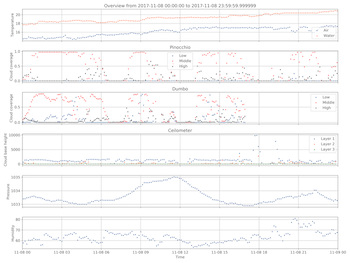
\includegraphics[width=\linewidth]{figures/overview.png}
	\end{minipage}%
	\begin{minipage}{.5\textwidth}
  		\centering
  		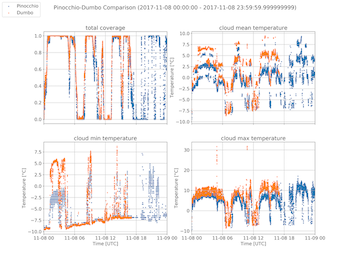
\includegraphics[width=\linewidth]{figures/comparison.png}
	\end{minipage}
	\caption{Overview and comparison plot.}
	\label{fig:plots}
\end{figure}
	
\end{enumerate}

\section{Cloud parameters}
\label{sec:cloud-parameters}
The main goal of SACIS is to calculate parameters from cloud images and retrieve further climate statistics. With \texttt{processor.py} one can calculate basic cloud parameters which are saved in the statistics files (where they should be saved can be set via \config{instrument}{stats}). All cloud parameters are available for three different height levels:
\begin{itemize}
	\item Level 1 - Low clouds: All clouds with a base height up to 2 km.
	\item Level 2 - Middle high clouds: All clouds with a base height from to 2 to 6 km.
	\item Level 3 - High clouds: All clouds with a base height higher than 6 km.
\end{itemize}

The cloud base height is retrieved by using a temperature gradient. At the moment, the temperature gradient is simply a lapse rate which provides a linear temperature descent (no inversions included). You can set the lapse rate via the config key \config{General}{lapse\_rate}.

\subsection{cloud\_coverage}
The cloud coverage $CC$ is the ratio between the number of cloud pixels and the total number of all unmasked pixel of the image:

\begin{equation}
	CC = \frac{n_\text{cloud}}{n_\text{all}} \qquad [0 - 1]
\end{equation}

\subsection{cloud\_inhomogeneity}
The cloud inhomogeneity $CI$ is a number to quantity the jaggedness of the clouds. It is defined by the perimeter of the clouds divided by their area:

\begin{equation}
	CI = \frac{p_\text{cloud}}{A_\text{cloud}} \qquad [0 - \infty]
\end{equation}

Please note that this parameter is very experimental and may be influenced by image size and the used mask.

\subsection{cloud\_mean\_temperature}
The cloud mean temperature $CT_\text{mean}$ is the mean temperature of all cloud pixels.

\subsection{cloud\_max\_temperature}
The cloud max temperature $CT_\text{max}$ is the maximum temperature of all cloud pixels.

\subsection{cloud\_min\_temperature}
The cloud min temperature $CT_\text{min}$ is the minimum temperature of all cloud pixels.

\section{Calibration of Pinocchio}
\label{sec:calibration}
Since the current script for calibration file generation, \texttt{pinocchio\_calibration.py}, is deprecated, further instructions of how to do the calibration of a Pinocchio camera and how to generate a calibration file are missing here.

\section{Development of \cloud}
\label{sec:development}

\subsection{Developer documentation}
There is a HTML documentation of all used modules and classes which can be generated by \href{http://www.sphinx-doc.org/en/stable/install.html}{Sphinx}. Call these commands in the directory of your \cloud toolbox:

\texttt{\$ cd docs}\\
\texttt{\$ make html}\\

Now you can call the \texttt{build/html/index.html} file with your favourite browser.

\subsection{Code style and design}
I tried following the \href{https://google.github.io/styleguide/pyguide.html}{Coding Style Guide by Google}  which is based on modern Python coding practices. The code is object oriented to make its structure better maintainable and extendable. If you are not familiar with object oriented programming, \href{https://www.youtube.com/watch?v=ZDa-Z5JzLYM}{here} is a good youtube video as an introduction.\\

The files for each instrument are represented by \texttt{typhon.spareice.Dataset} objects (\href{http://radiativetransfer.org/misc/typhon/doc-trunk/tutorials/dataset.html}{link} to further documentation and tutorial). I developed those objects to make handling and processing of datasets with many files easier and faster. \texttt{typhon.spareice.Dataset} is still under development and may change its API and name in future. When those major changes come, I will contact you so that the \cloud toolbox can be developed and still benefit from typhon updates.

%\subsection{Modules}
%The scripts from section \ref{sec:scripts} mainly call functions from modules. If you want to develop the \cloud toolbox, you should modify the modules rather than the scripts. They are located in the \texttt{cloud} folder.
%\begin{table}[h!]
%	\centering
%	\begin{tabular}{|l|l|}
%	\hline 
%	\textbf{Module} & \textbf{Description}\\ 
%	\hline \hline 
%	\texttt{image.py} & \tabitem Converts pinocchio files from jpg to netcdf format and\\ 
%	& applies calibration.\\
%	& \tabitem Applies mask on pinocchio images.\\
%	& \tabitem Calculates cloud statistics from pinocchio images.\\ 
%	\hline 
%	\texttt{pinocchio\_calibration.py} &  \tabitem Creates calibration file from pinocchio images \\
%	& (see section FIXME)\\ 
%	\hline 
%	\texttt{dumbo\_workflow.py} & \tabitem Converts dumbo files from ascii to netcdf format.\\
%	& \tabitem Applies mask on dumbo images.\\
%	& \tabitem Calculates cloud statistics from dumbo images.\\ 
%	\hline 
%	\texttt{monitor.py} & \tabitem Produces overview and comparison plots for all components.\\ 
%	\hline 
%	\end{tabular} 
%\end{table}
\end{document}